In this chapter we evaluate DaisyNFS and GoTxn along the dimensions of
performance, correctness, and functionality.

\section{Performance}
\label{sec:eval:bench}

To evaluate the performance of DaisyNFS, we ran three benchmarks: the LFS smallfile
and largefile benchmarks, and a development workload that consists of \cc{git
clone} from a local repository followed by running \cc{make}. These are the same
benchmarks used by DFSCQ~\cite{chen:dfscq} (a state-of-the art sequential
verified file system) and for an unverified NFS server implemented on top of
GoJournal~\cite{chajed:gojournal}. As a baseline, this evaluation uses a Linux
NFS server exporting an ext4 file system mounted with \cc{data=journal} mode.
The NFS server lets us compare fairly since both go through the Linux NFS client
and use the same underlying protocol. Using \cc{data=journal} forces all data to
go through the journal and disables log-bypass writes, which ensures that
ext4 and DaisyNFS both guarantee NFS RPCs are committed durably when they return. In
\cc{data=ordered} mode Linux achieves better performance but can
lose recently written data if the system crashes.

All of these benchmarks were run using Linux~5.13 and Go~1.18 on an Amazon
EC2 i3.metal instance, which has 72 cores, 512~GB of RAM, and a local 1.9~TB
NVMe SSD.\@ To reduce variability we limit the experiment to a single 36-core
socket, disable turbo boost, and disable processor sleep states; the coefficient
of variation for all experiments is under 5\% so we omit error bars for visual
clarity.

%% cpupower frequency-set -g performance
%% threads=32 in the [nfsd] section of /etc/nfs.conf

%% SINGLE-CORE EXPERIMENTS:
%%   for n in $(seq 8 15) $(seq 24 31); do echo 0 > /sys/devices/system/cpu/cpu$n/online; done

\begin{figure}
  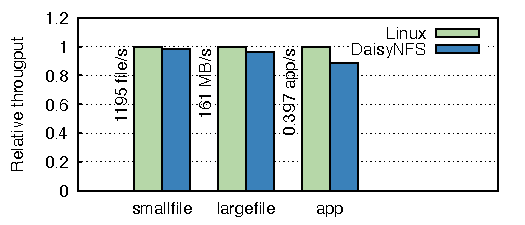
\includegraphics{daisy-nfs/fig/bench.pdf}
  \caption[Performance for smallfile, largefile, and app benchmarks]%
  {Performance of Linux NFS and DaisyNFS for \cc{smallfile},
    \cc{largefile}, and \cc{app} workloads, on an NVMe disk.
    DaisyNFS achieves comparable performance to ext4 in \cc{data=journal} mode.}
  \label{fig:eval:bench}
\end{figure}

The results are shown in \cref{fig:eval:bench}. DaisyNFS gets about the same
throughput as Linux on the smallfile benchmark, which is intended to
be metadata-heavy. The smallfile benchmark repeatedly creates a file,
writes 100 bytes to it and syncs the file, then deletes it.

DaisyNFS gets slightly better throughput compared to Linux on the largefile benchmark, which is
intended to measure bulk data writes. Note that in this benchmark ext4 would be
significantly faster in \cc{data=ordered} mode due to no longer writing all data
through the journal; with that option it gets 315~MB/s even over
NFS.\@ The largefile benchmark creates a 300~MB file by appending repeatedly, then
syncs it. The Linux NFS client buffers the entire append process until the final
sync, at which point it issues the writes in many chunks in parallel. This
benchmark is challenging to support efficiently because the writes at the NFS
server do not come in order, so some are past the end of the file. The semantics
of such a write are to fill the gap with zeros, but both DaisyNFS and Linux get good
performance despite this because they implicitly encode those zeros without even
allocating a block. DaisyNFS gets comparable performance on this benchmark because
GoTxn is good at handling concurrent synchronous writes.

DaisyNFS achieves good performance on the app workload, which consists of running
\cc{git clone} on the xv6 repository followed by \cc{make}. xv6 is an operating
system, so building it requires running the usual development tools---gcc, ld,
ar---but also running dd to generate a kernel image. Builds take about 3s,
which are reported as a throughput number so higher is better.

\section{Scalability}
\label{sec:eval:scale}

DaisyNFS executes NFS operations concurrently to achieve better performance with
multiple cores. This section evaluates the scalability of the whole system,
especially the concurrency provided by GoTxn. The benchmark used is the smallfile benchmark from
\cref{sec:eval:bench}, with a varying number of cores. Because this experiment runs
on a physical disk, other threads have a chance to prepare transactions while the
transaction system is committing to disk.

\begin{figure}
  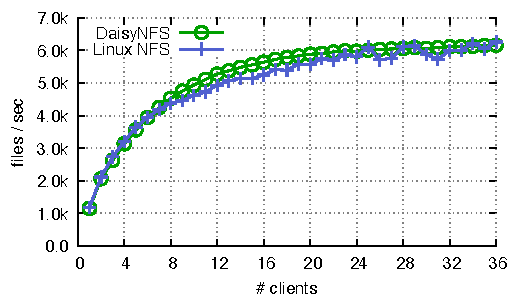
\includegraphics{daisy-nfs/fig/scale.pdf}
  \caption[Concurrent smallfile performance]%
{Combined throughput of the \cc{smallfile} microbenchmark running on
    an NVMe drive while
    varying the number of concurrent clients. DaisyNFS's performance scales with the
    number of cores similar to ext4; both eventually saturate the disk and scale
    sub-linearly.}
  \label{fig:eval:scale}
\end{figure}

The results are shown in \cref{fig:eval:scale}. The graph shows that DaisyNFS
achieves both good absolute performance and gets higher throughput with more
clients, comparable to the scalability of the Linux NFS server.
DaisyNFS scales slightly sub-linearly due to a lock in GoTxn's object layer that
serializes installation of writes into disk blocks at commit time.

\section{Testing the trusted code and spec}

For the proof of \cref{thm:daisy-correctness} to apply to the actual server, we trust that (1) the
Dafny code is a ``safe'' use of the transaction system, (2) sequential
refinement is correctly encoded into Dafny, (3) the libraries for Go primitives
are correctly specified in Dafny, and (4) the unverified Go code calling the
Dafny methods and implementing the NFS wire protocol is correct. The
user must follow the assumed execution model and run initialization from an
empty disk and recovery after each boot. Finally, the disk needs to behave
according to its assumed specification, which requires that it preserve written
data and not corrupt it.

Beyond satisfying this formal theorem statement, we want two more things from
the implementation and specification: first that the specification as formalized
actually reflects the RFC, and second we would like DaisyNFS to be compatible
with existing clients, including implementing enough of the RFC's functionality.
These fall outside the scope of verification so we cover them with testing.

To evaluate the file system, we mounted it using the Linux NFS client and ran the
fsstress and fsx-linux tests, two suites used for testing the Linux kernel. In
order to look for bugs in crash safety and recovery, we also ran
CrashMonkey~\cite{mohan:crashmonkey}, which found no bugs
after running all supported 2-operation tests.

While other experiments in the evaluation interact with DaisyNFS via the Linux
client, these tests interact with the server directly from a hand-written
client. That client is then tested with symbolic execution, with feedback from
the entire machine.\footnote{The framework for this testing is part of an
unrelated research project so we don't give details on the methodology here.}
This testing produces a wider range of requests than are possible via the Linux
client. The process helped us find and fix several bugs in the unverified parts
of DaisyNFS and in the specification itself, which are reported in
\cref{fig:daisynfs-bugs}.

Two of the specification bugs are particularly interesting. The bounded inode bug
was due to an \cc{ino} argument of type \cc{Ino}; this type is a Dafny
\emph{subset type}, thus adding an implicit precondition that \cc{ino <
NUM_INODES}, which can be violated by the (unverified) Go code. The fix is to instead
use a \cc{uint64} and check the bound in verified code. The RENAME bug was due
to having an incomplete specification (and implementation) that did not capture
that RENAME should only overwrite when the source and destination are
compatible.

\begin{figure}
  \begin{center}
  \begin{tabular}{@{}p{8cm}p{2.7cm}@{}}
    \toprule
    \textbf{Bug} & \textbf{Why?} \\
    \midrule
    XDR decoder for strings can allocate $2^{32}$ bytes & Unverified \\
    File handle parser panics if wrong length & Unverified \\
    WRITE panics if not enough input bytes & Unverified \\
    Directory REMOVE panics in dynamic type cast & Unverified \\
    Panic on unexpected enum value & Unverified \\
    The names \cc{.} and \cc{..} are allowed & Not in RFC 1813 \\
    RENAME can create circular directories & Not in RFC 1813 \\
    CREATE/MKDIR allow empty name & Specification \\
    Proof assumes caller provides bounded inode & Specification \\
    RENAME allows overwrite where spec does not & Specification \\
    \bottomrule
  \end{tabular}
  \end{center}
  \caption{Bugs found by testing at the NFS protocol level.}
  \label{fig:daisynfs-bugs}
\end{figure}

%As a sanity check on the transaction system, we fuzzed the interface presented
%to Dafny using a test harness capable of performing arbitrary reads, writes and
%commits while following the transaction system's preconditions. The test checks
%that the transaction system does not crash and returns the correct data on read.
%The fuzzing did generate complex inputs with multiple chained operations but did
%not find any bugs, but we note that our fuzzing is limited to
%single-threaded and crash-free behavior. \joe{I think we could cut this para now, or perhaps make it more focused by saying it's about testing the trusted boundary between Dafny and GoTxn. But I'm not quite sure it actually does test that?}

\section{Incremental improvements}
\label{sec:eval:incremental}

\begin{figure}
\begin{center}
\begin{tabular}{lrr}
  \toprule
  \textbf{Feature} & \textbf{Time} & \textbf{Lines} \\
  \midrule
  In-place directory updates & 2 days & 600\\
  Multi-block directories & 5 days & 800 \\
  NFS attributes & 4 days & 500 \\
  Freeing space (\cref{sec:dafny:freeing}) & 3 days & 1400\\
  \bottomrule
\end{tabular}
\end{center}
\caption{Incremental improvements were implemented quickly and without much
  code (which includes both implementation and proof).}
\label{fig:features}
\end{figure}

DaisyNFS was implemented and verified over the course of three months by
one of the authors, until it had support for enough of NFS to run. We
added several features incrementally after the initial prototype
worked, both to improve performance and to support more
functionality. Some of the interesting changes are listed in
\cref{fig:features}.  To improve performance, we switched to
operating on the serialized representation of directories directly
(decoding fields on demand and encoding in-place) and then added also
multi-block directories.  We added support for attributes so that the file
system stores the mode, uid/gid, and modification timestamp for files and directories.
Finally, we implemented the freeing plan described
in \cref{sec:dafny:freeing}, which required additional code through the
whole stack (but by design no changes to the file-system invariant).
We believe additional features such as symbolic links
could be added incrementally with modest effort because
of sequential reasoning and proof automation.

%% \begin{itemize}
%%   \item Directories were initially parsed into a functional data structure, then
%%   re-serialized to make changes. To improve performance, we switched to
%%   operating on the serialized representation directly (decoding fields on demand
%%   and encoding in-place). (2 days, 600 lines changed)
%%   \item Single-block directories were too limiting, so we switched to multiple
%%   blocks, which are read into memory on demand. We still operate on the
%%   serialized representation, but now of only part of the directory. (5 days, 800
%%   lines changed)
%%   \item Initially we only tracked file types. We added support for attributes so
%%   that the mode, uid/gid, and modification timestamp would be stored correctly.
%%   (4 days, 500 lines changed)
%%   \item The file system initially only freed the first 8 direct blocks of an
%%   inode. We implemented the space-freeing plan described in
%%   \cref{sec:dafny:freeing} through the whole stack afterward. (3 days, 1400
%%   lines changed)
%% \end{itemize}
